% Options for packages loaded elsewhere
\PassOptionsToPackage{unicode}{hyperref}
\PassOptionsToPackage{hyphens}{url}
%
\documentclass[
]{article}
\usepackage{amsmath,amssymb}
\usepackage{lmodern}
\usepackage{iftex}
\ifPDFTeX
  \usepackage[T1]{fontenc}
  \usepackage[utf8]{inputenc}
  \usepackage{textcomp} % provide euro and other symbols
\else % if luatex or xetex
  \usepackage{unicode-math}
  \defaultfontfeatures{Scale=MatchLowercase}
  \defaultfontfeatures[\rmfamily]{Ligatures=TeX,Scale=1}
\fi
% Use upquote if available, for straight quotes in verbatim environments
\IfFileExists{upquote.sty}{\usepackage{upquote}}{}
\IfFileExists{microtype.sty}{% use microtype if available
  \usepackage[]{microtype}
  \UseMicrotypeSet[protrusion]{basicmath} % disable protrusion for tt fonts
}{}
\makeatletter
\@ifundefined{KOMAClassName}{% if non-KOMA class
  \IfFileExists{parskip.sty}{%
    \usepackage{parskip}
  }{% else
    \setlength{\parindent}{0pt}
    \setlength{\parskip}{6pt plus 2pt minus 1pt}}
}{% if KOMA class
  \KOMAoptions{parskip=half}}
\makeatother
\usepackage{xcolor}
\usepackage[margin=1in]{geometry}
\usepackage{graphicx}
\makeatletter
\def\maxwidth{\ifdim\Gin@nat@width>\linewidth\linewidth\else\Gin@nat@width\fi}
\def\maxheight{\ifdim\Gin@nat@height>\textheight\textheight\else\Gin@nat@height\fi}
\makeatother
% Scale images if necessary, so that they will not overflow the page
% margins by default, and it is still possible to overwrite the defaults
% using explicit options in \includegraphics[width, height, ...]{}
\setkeys{Gin}{width=\maxwidth,height=\maxheight,keepaspectratio}
% Set default figure placement to htbp
\makeatletter
\def\fps@figure{htbp}
\makeatother
\setlength{\emergencystretch}{3em} % prevent overfull lines
\providecommand{\tightlist}{%
  \setlength{\itemsep}{0pt}\setlength{\parskip}{0pt}}
\setcounter{secnumdepth}{-\maxdimen} % remove section numbering
\ifLuaTeX
  \usepackage{selnolig}  % disable illegal ligatures
\fi
\IfFileExists{bookmark.sty}{\usepackage{bookmark}}{\usepackage{hyperref}}
\IfFileExists{xurl.sty}{\usepackage{xurl}}{} % add URL line breaks if available
\urlstyle{same} % disable monospaced font for URLs
\hypersetup{
  hidelinks,
  pdfcreator={LaTeX via pandoc}}

\author{}
\date{\vspace{-2.5em}}

\begin{document}

\hypertarget{team-project-1}{%
\section{Team-Project-1}\label{team-project-1}}

\textbf{Partner names: Abizer Mamnoon, Luis Gomez}

\hypertarget{data}{%
\subsection{Data}\label{data}}

The data \texttt{MonthlyWeather.csv} contain monthly weather readings
for 113 US airports from July, 2014 through September, 2017. Variable
descriptions are given below. The location of this data is
\url{https://raw.githubusercontent.com/mgelman/data/master/MonthlyWeather.csv}.

\hypertarget{to-do}{%
\subsection{To do:}\label{to-do}}

Use \texttt{ggplot2} to create graphs that can answer the following
questions. For each set of questions, create 1-2 graphs and use the
graphs to answer the questions in a paragraph or two. You will be graded
on the appropriateness and originality of your graphs,
explanation/interpretation, and the readability of your R code.

\begin{enumerate}
\def\labelenumi{\arabic{enumi}.}
\tightlist
\item
  Suppose you don't like big daily temperature swings and cloudy days.
  Which month(s) or time of year have the most consistent daily temps?
  the most variable daily temps? Which month(s) or time of year have the
  most sunny days? the fewest sunny days?
\end{enumerate}

\#The code below depicts a bar graph of the average temperature range
vs.~months. The bar graph is arranged in decending order from the month
with the highest temperature range to the lowest.

\begin{verbatim}
## Warning: Removed 1 rows containing missing values (position_stack).
\end{verbatim}

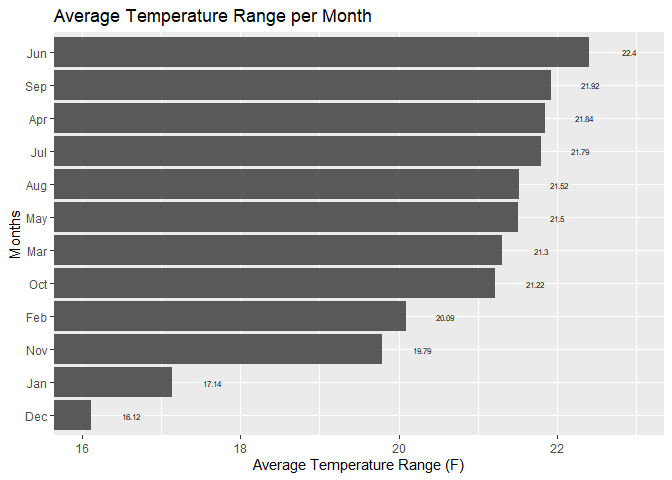
\includegraphics{FinalProject_files/figure-latex/unnamed-chunk-2-1.pdf}

December has the most consistent daily temperature as the average of the
daily max - min temperature in June is the lowest at 16.1 degrees F.
June has the most variable daily temperatures as the average of the
daily max - min temperature in June is the highest at 22.4 degrees
F.Based on the graph, September is somewhat of an outliar since it is
equal to 0.

\#The code below depicts a bar graph of the mean number of sunny day
vs.~months. The bar graph is arranged in decending order from the month
with the most days of sunny days to the lowest.
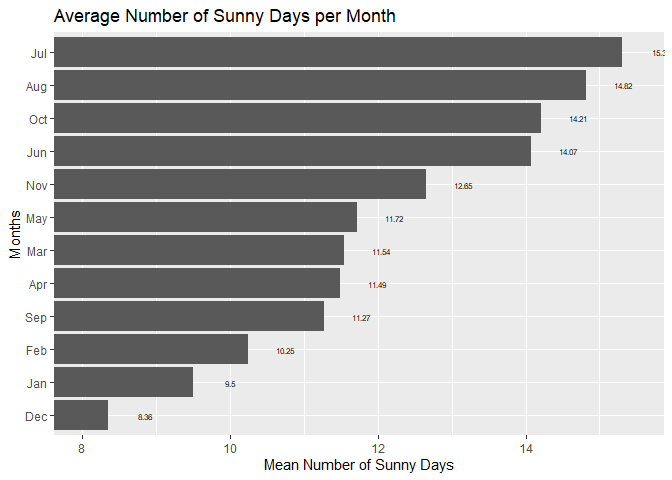
\includegraphics{FinalProject_files/figure-latex/unnamed-chunk-3-1.pdf}

December has on average 8.4 sunny days which is the lowest average
number of sunny days a month has in the year. July has on average 15.3
sunny days which is the highest average number of sunny days a month has
in the year.

\begin{enumerate}
\def\labelenumi{\arabic{enumi}.}
\setcounter{enumi}{1}
\tightlist
\item
  Consider 2016 weather data. Which regions or states have the most
  consistent daily temps? the most variable daily temps? Which regions
  or states have the most sunny days? the fewest sunny days?
\end{enumerate}

\#The code below depicts a map of the US and its average temperature
range in 2016. Each US state in the map is colored with a shade of
orange that represents a temperature range. The higher the number, the
darker the shade of orange the state will be.\\
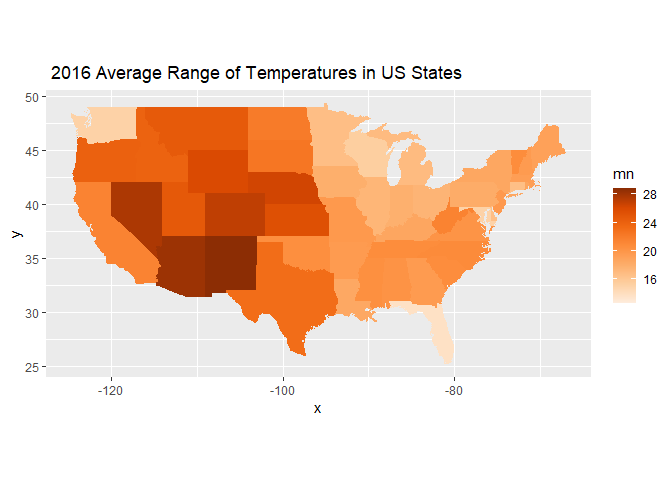
\includegraphics{FinalProject_files/figure-latex/unnamed-chunk-4-1.pdf}

States in the East have more consistent temperatures than states in the
West.There are more variable sunny days in the West. Florida is the
state with the lowest average temperature range while New Mexico is
state with the most highest average temperature range.

\#The code below depicts a map of the US and its average number of sunny
days range in 2016. Each US state in the map is colored with a shade of
purple that represents a number of sunny days. The higher the number,
the darker the shade of purple the state will be.\\
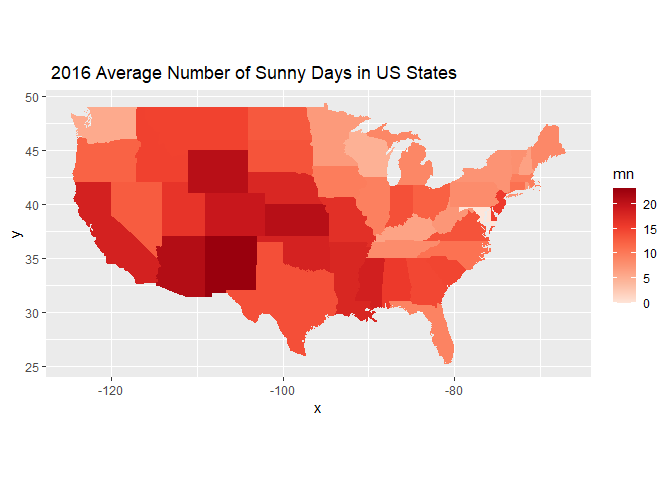
\includegraphics{FinalProject_files/figure-latex/unnamed-chunk-5-1.pdf}
States in the central part of the US tend to have more sunny days. While
states in the midwest and North East tend to have the least number of
sunny days. New Mexico has the most average number of sunny days while a
state in the North East is the state with the lowest number of sunny
days.

\begin{enumerate}
\def\labelenumi{\arabic{enumi}.}
\setcounter{enumi}{2}
\tightlist
\item
  What criteria are important to you for choosing a city to live in?
  Create some figures that help determine which city you would live in
  based on that criteria. Would you choose one particular city to live
  in year round or would you migrate to different locations depending on
  the season?
\end{enumerate}

\#The code below depicts a map of the US and its average number of sunny
days range in 2016. Each US state in the map is colored with a shade of
blue that represents a number of average minimum temperature. The higher
the number, the darker the shade of blue the state will be.

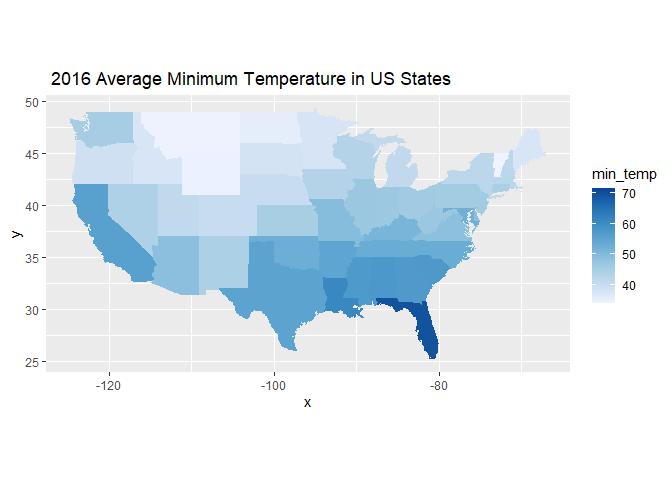
\includegraphics{FinalProject_files/figure-latex/unnamed-chunk-7-1.pdf}
States in the Northern part of the US tend to have a lower average
number of minimum temperature while states in the south tend to have a
higher average number of temperature.

\#The code below depicts a map of the US and its average number of
percipitation in 2016. Each US state in the map is colored with a shade
of blue that represents a number of amount of percipitation. The higher
the number, the darker the shade of blue the state will be.
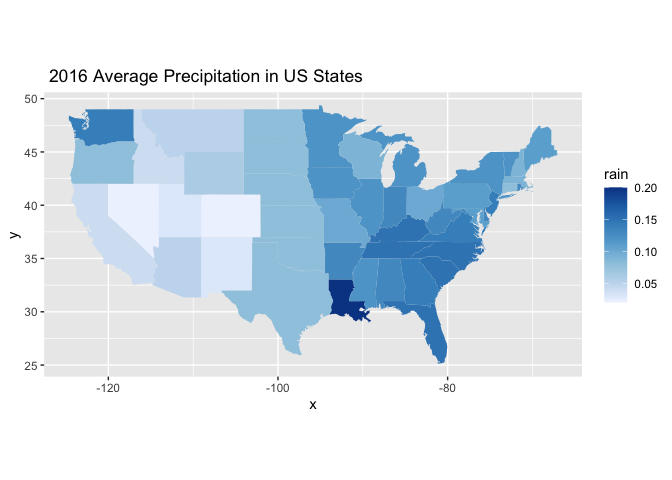
\includegraphics{FinalProject_files/figure-latex/unnamed-chunk-8-1.pdf}
States in the south west part of the US tend to have the most average
amount of precipitation, with Louisiana having the most. States in the
Western part of the US tend to have the least amount of precipitation.

\#The code below depicts a map of the US and its average number of wind
speed in 2016. Each US state in the map is colored with a shade of blue
that represents a number of wind speed. The higher the number, the
darker the shade of blue the state will be.
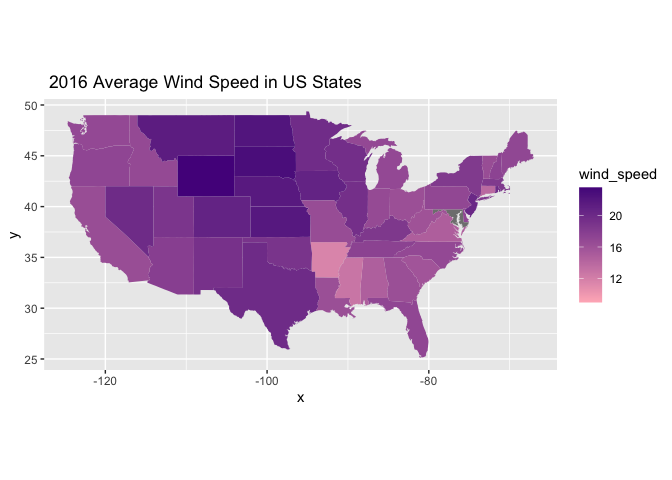
\includegraphics{FinalProject_files/figure-latex/unnamed-chunk-9-1.pdf}
States around Arkansas tend to have lower wind speeds. The place with
the most wind speed is Wyioming.

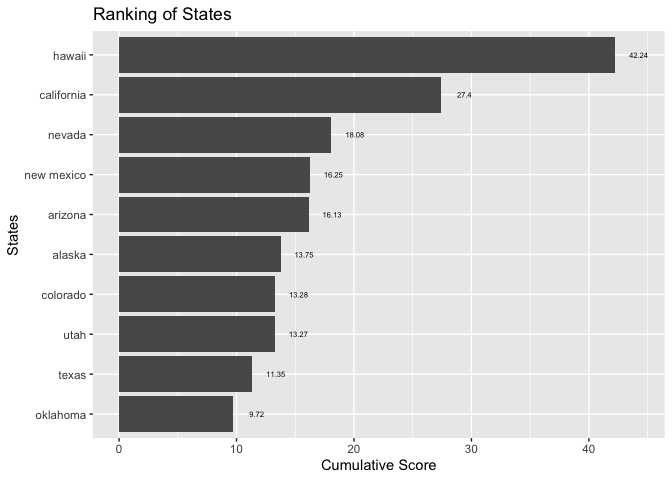
\includegraphics{FinalProject_files/figure-latex/unnamed-chunk-10-1.pdf}
The equation we came up with goes as follows: as minimum temperature
increases the rating increases, for wind speed there is a negative
relation as the higher the wind speed the lower the rating, for rain we
multiplied the variable by 300 in order to make it the same range as the
rest (also negative relation). According to our bar graph, Hawaii is the
best place to live in.

\hypertarget{turn-in}{%
\subsection{Turn in:}\label{turn-in}}

Push your .Rmd and .md to GitHub by Tue, Sep.~27 11:59PM. Hide all code
in your knitted doc so I just see graphs, interpretations, and section
headers for each part.

\hypertarget{variables}{%
\subsection{Variables:}\label{variables}}

\begin{itemize}
\tightlist
\item
  \texttt{avgMinTmpF} and \texttt{avgMaxTmpF} average of daily max or
  min temps
\item
  \texttt{minTmpF} and \texttt{maxTmpF} monthly min or max temps
\item
  \texttt{avgTmpF} average temp
\item
  \texttt{avgTmpDiffF} mean of daily max - min temps
\item
  \texttt{avgPrecipIn} average daily precipitation (inches)
\item
  \texttt{maxWindMPH} monthly max sustained wind speed
\item
  \texttt{avgWindMPH} average of daily max sustained wind speed
\item
  \texttt{numSunDay} number of days that are clear/mostly sunny
\item
  \texttt{numDay} number of measured days
\item
  \texttt{AirPtCd} airport code
\item
  \texttt{city} closest city to the airport
\item
  \texttt{state} location of airport
\item
  \texttt{latitude}, \texttt{longitude}
\item
  \texttt{month}, \texttt{year}
\end{itemize}

\hypertarget{grading-66-points-possible-22part}{%
\subsection{Grading: 66 points possible
(22/part)}\label{grading-66-points-possible-22part}}

Each part above (1-3) will have a score determined by: score =
2*correctness + design + presentation + style

5 point scale for

\begin{itemize}
\tightlist
\item
  correctness: does code work and produce results that address the
  desired goal
\item
  design and originality: does the graph effectively display information
  and provide context, and/or does it convey info in a unique way
\item
  presentation: does your written explanation effectively motivate and
  explain your analysis

  \begin{itemize}
  \tightlist
  \item
    5 = best, basically no room for improvement
  \item
    4 = better, minor room for improvement
  \item
    3 = good, some room for improvement
  \item
    2 = fair, ample room for improvement
  \item
    1 = poor, did not finish
  \item
    0 = no attempt
  \end{itemize}
\end{itemize}

Two-point scale for

\begin{itemize}
\tightlist
\item
  style and readability: is the code readable and appropriately
  commented

  \begin{itemize}
  \tightlist
  \item
    2 = readable and sufficient comments
  \item
    1 = mostly readable but contains one or more portions that could be
    written in a more clear manner
  \item
    0 = most code could be written in a more readable manner
  \end{itemize}
\end{itemize}

\end{document}
